%
\documentclass[tikz]{standalone}

\usepackage{tikz}
\usetikzlibrary{calc}
\usetikzlibrary{lindenmayersystems}

\begin{document}
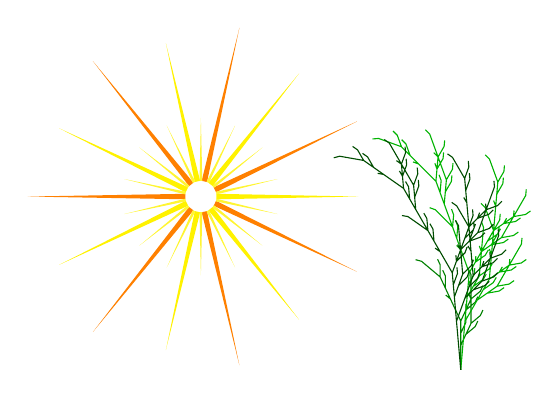
\begin{tikzpicture}



%% Zweig
\begin{scope}[xshift=3.3cm,yshift=-2.2cm, scale=1.1]
\pgfdeclarelindenmayersystem{Fractal plant}{
  \rule{X -> F-[[X]+X]+F[+FX]-X}
  \rule{F -> FF}
%  \rule{X -> F[X]}  
  }

    \draw [green!50!black, rotate=90]
    [l-system={Fractal plant, axiom=X, order=3, step=2pt, angle=25}]
    lindenmayer system; 
    \draw [green!70!black, rotate=85]
    [l-system={Fractal plant, axiom=X, order=4, step=2pt, angle=25}]
    lindenmayer system; 
    \draw [green!30!black, rotate=95]
    [l-system={Fractal plant, axiom=X, order=4, step=2pt, angle=25}]
    lindenmayer system; 
\end{scope}


%% Star

\newcommand{\drawstar}[1]{
\foreach \i in {1,...,\nstar}{
	\pgfmathsetmacro{\ang}{360*\i/\nstar+\rot}
	\path (C)++(\ang+\dangi:\Ri) coordinate(L);
	\path (C)++(\ang-\dangi:\Ri) coordinate(R);
	\path[fill=#1] (L)--($(C)+(\ang:\Ro)$) -- (R);
}}



\path (0,0) coordinate(C);
\def\nstar{7}
\def\Ri{.2}
\def\Ro{2}
\def\dangi{10}
\def\rot{0}
\drawstar{yellow};

\def\Ro{2.2}
\pgfmathsetmacro{\rot}{360/7/2}
\drawstar{orange};

\def\nstar{14}
\def\Ro{1}
\def\dangi{5}
\pgfmathsetmacro{\rot}{360/7/4}
\drawstar{yellow!80};









\end{tikzpicture}
\end{document} 
